\documentclass[hyperref={bookmarks=false},aspectratio=169]{beamer}
\usepackage{hyperref,ragged2e,amsmath,amssymb,url,bm}
\usepackage{graphicx,booktabs,array}
\usepackage{tikz}
\usetikzlibrary{arrows.meta,positioning,calc,shapes.geometric,decorations.pathreplacing,matrix}
\graphicspath{{crops/}}
\usetheme{Goettingen}
% --- Paleta: azul profundo, dorado y papiro crema ---
\definecolor{azul}{HTML}{15437C}
\definecolor{azuloscuro}{HTML}{0B1F3A}
\definecolor{celeste}{HTML}{5694D6}
\definecolor{dorado}{RGB}{196,154,60}
\definecolor{papiro}{RGB}{246,239,220}
\definecolor{gris}{RGB}{70,78,96}
\setbeamercolor{structure}{fg=azul}
\setbeamertemplate{sidebar canvas right}[vertical shading][top=azul,bottom=azuloscuro]
\setbeamercolor{title in sidebar}{fg=dorado}
\setbeamercolor{author in sidebar}{fg=papiro}
\setbeamercolor{section in sidebar}{fg=papiro}
\setbeamercolor{section in sidebar shaded}{fg=dorado!70!papiro}
\setbeamercolor{subsection in sidebar}{fg=papiro}
\setbeamercolor{subsection in sidebar shaded}{fg=dorado!70!papiro}
\let\raggedright\justifying
\setlength{\RaggedRightRightskip}{0pt plus 1fil}
\setbeamertemplate{background canvas}{
\includegraphics[width=\paperwidth,height=\paperheight]{papiro.jpg}}
\setbeamercolor{normal text}{fg=black!88!azuloscuro}
\setbeamercolor{frametitle}{fg=azul}
\setbeamerfont{frametitle}{series=\bfseries}
\setbeamertemplate{section in toc shaded}{\leavevmode{\color{gris}\inserttocsection}\par}
\setbeamercolor{title}{fg=azul}
\setbeamercolor{subtitle}{fg=gris}
\setbeamercolor{item projected}{bg=azul,fg=papiro}
\setbeamertemplate{itemize item}{\small\textcolor{dorado}{$\blacktriangleright$}}
\setbeamertemplate{navigation symbols}{}
% --- Español + hebreo + griego (XeLaTeX) ---
\usepackage[bidi=default]{babel}
\babelprovide[import,main]{spanish}
\babelprovide[import]{hebrew}
\babelprovide[import]{ancientgreek}
\babelfont[hebrew]{sf}[Path=fonts/, BoldFont=NotoHebrewSans-700.ttf]{NotoHebrewSans-400.ttf}
\babelfont[hebrew]{rm}[Path=fonts/, BoldFont=NotoHebrewSans-700.ttf]{NotoHebrewSans-400.ttf}
\babelfont[ancientgreek]{sf}[Path=fonts/]{GFSPorson.otf}
\babelfont[ancientgreek]{rm}[Path=fonts/]{GFSPorson.otf}
\newcommand{\heb}[1]{\mbox{\foreignlanguage{hebrew}{#1}}}
\newcommand{\grc}[1]{\foreignlanguage{ancientgreek}{#1}}
\newcommand{\SENOR}{S{\fontsize{0.78em}{1em}\selectfont EÑOR}}
% --- Citas (cuadro de un solo color), imágenes, referencias ---
\usepackage[most]{tcolorbox}
\newtcolorbox{cita}[1][]{enhanced, colback=azul!7!papiro, opacityback=0.85, colframe=azul,
  boxrule=0pt, leftrule=2.5pt, arc=0pt, left=6pt, right=6pt, top=4pt, bottom=4pt,
  before skip=4pt, after skip=6pt, fontupper=\small\itshape, #1}
\newcommand{\fuente}[1]{\par\hfill{\upshape\bfseries\footnotesize\textcolor{azul}{#1}}}
\makeatletter
\newcommand{\fotolado}[2]{%
  \begin{tikzpicture}[remember picture,overlay]
    \node[anchor=north east,inner sep=0pt] (foto) at ([xshift=-\beamer@sidebarwidth]current page.north east)
      {\includegraphics[height=\paperheight]{#1}};
    \node[anchor=south east,inner sep=2pt,text=papiro,fill=azuloscuro,fill opacity=0.6,text opacity=1,
      font=\fontsize{4.5}{5.5}\selectfont,align=right,text width=4.2cm] at ([xshift=-3pt,yshift=3pt]foto.south east)
      {\textit{Nota.} #2};
  \end{tikzpicture}}
\makeatother
\newcommand{\refapa}[1]{\par{\RaggedRight\hangindent=1.2em\hangafter=1\noindent #1\par}\vspace{3pt}}
\usepackage{xurl}\urlstyle{same}
\newcommand{\destacar}[1]{\textbf{\textcolor{azul}{#1}}}
\newcommand{\precision}[1]{{\footnotesize\color{gris}\textbf{Precisión:} #1}}
\tikzset{caja/.style={draw=azul,line width=0.8pt,fill=papiro,fill opacity=0.92,text opacity=1,rounded corners=3pt,inner sep=5pt,font=\scriptsize}}
\usepackage{qrcode}
% engranaje: centro, radio, dientes, color
\newcommand{\gear}[4]{\fill[#4] #1 circle (#2);
  \foreach \k in {1,...,#3}{\pgfmathsetmacro{\a}{360/#3*\k}
    \fill[#4,rotate around={\a:#1}] ($#1+(-0.09,#2-0.02)$) rectangle ($#1+(0.09,#2+0.16)$);}}
\title[Dios es uno]{\bfseries{Dios es uno}}
\subtitle{``Oye, Israel: \SENOR{} nuestro Dios, \SENOR{} uno es'' (Dt 6:4)}
\author{}\institute{}\date{}
\titlegraphic{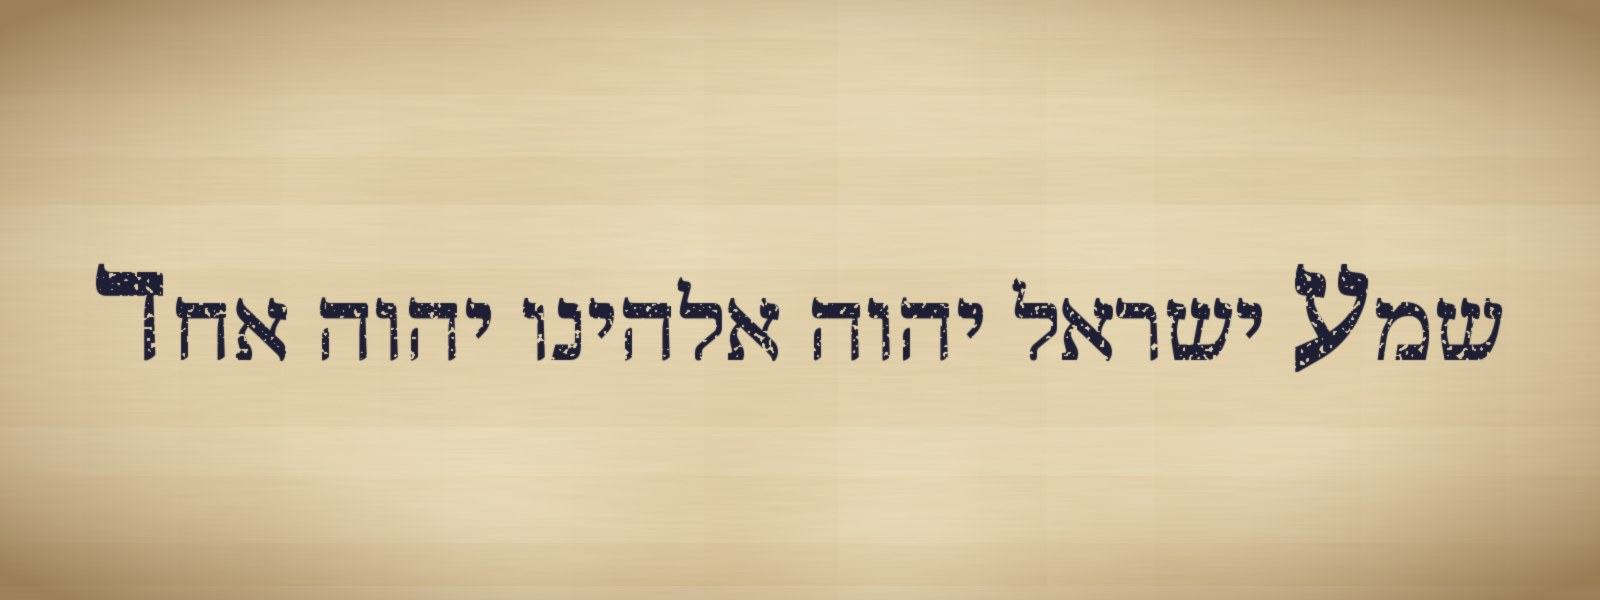
\includegraphics[width=0.80\linewidth,height=0.36\textheight,keepaspectratio]{portada.jpg}\\[-1pt]
  {\fontsize{5}{6}\selectfont\color{gris}\textit{Nota.} Elaboración propia: Dt 6:4 en texto hebreo consonántico (BHS), con la \emph{ayin} y la \emph{dálet} grandes de la tradición masorética.}}
\begin{document}
\frame{\titlepage}

\begin{frame}\frametitle{Contenidos}\tableofcontents\end{frame}

% ------------------------------------------------------------------
\section{Contexto}

\begin{frame}{``Que yo soy \SENOR''}
\begin{cita}Así dijo \SENOR: No se alabe el sabio en su sabiduría, ni en su valentía se alabe el valiente, ni el rico se alabe en sus riquezas. Mas alábese en esto el que se hubiere de alabar: en entenderme y conocerme, que yo soy \SENOR, que hago misericordia, juicio y justicia en la tierra; porque estas cosas quiero, dice \SENOR.\fuente{(Jer 9:23--24 [9:22--23], RVR1960)}\end{cita}
\begin{center}\heb{הַשְׂכֵּל וְיָדֹעַ אוֹתִי כִּי אֲנִי יְהוָה}\end{center}
\small\RaggedRight Conocer a Dios empieza por una afirmación: \heb{אֲנִי יְהוָה}, ``yo soy \SENOR''. La misma fórmula sostiene la confesión de Isaías: ``Yo soy \SENOR, y ninguno más hay'' (Is 45:5). Antes de saber \emph{cómo} es Dios, Israel aprende \emph{cuántos} dioses hay: uno.
\end{frame}

\begin{frame}{La pregunta del atributo}
\begin{columns}[c,onlytextwidth]
\begin{column}{0.52\textwidth}
\begin{tcolorbox}[colback=papiro,colframe=azul,boxrule=1pt,arc=3pt]
\small\textbf{Unidad:} hay un solo Dios, y ese Dios es uno en sí mismo, sin rival, sin división y sin semejante.
\end{tcolorbox}
\begin{cita}A ti te fue mostrado, para que supieses que \SENOR{} es Dios, y no hay otro fuera de él.\fuente{(Dt 4:35, RVR1960)}\end{cita}
\begin{cita}Acordaos de las cosas pasadas desde los tiempos antiguos; porque yo soy Dios, y no hay otro Dios, y nada hay semejante a mí.\fuente{(Is 46:9, RVR1960)}\end{cita}
\end{column}
\begin{column}{0.46\textwidth}\small
\begin{itemize}
\item Con la preexistencia, abre la \destacar{Parte I (Ser)} y es el cimiento de los demás: todo lo que se diga de Dios se dice de \emph{uno}.
\item Israel lo confiesa con dos palabras: \heb{יְהוָה אֶחָד}, ``\SENOR{} uno''.
\item No lo aprendió en una escuela de filosofía, sino rodeado de dioses: Egipto, Canaán, Baal, Asiria y Babilonia.
\end{itemize}
\end{column}
\end{columns}
\end{frame}

\begin{frame}{Un atributo del Ser}
\centering
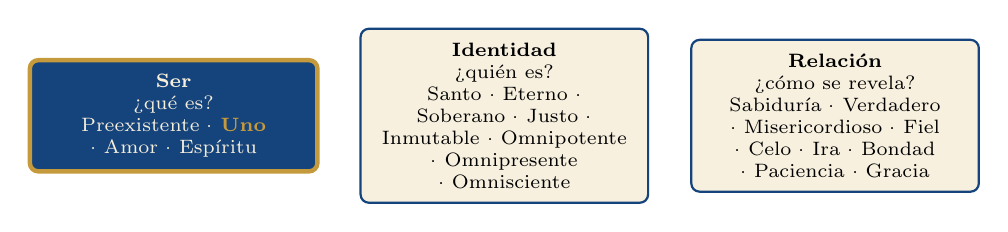
\begin{tikzpicture}[font=\scriptsize]
 \node[draw=dorado,line width=1.6pt,fill=azul,text=papiro,rounded corners=3pt,text width=3.3cm,align=center,inner sep=5pt] (s) at (-4.2,0) {\textbf{Ser}\\ ¿qué es?\\ Preexistente · \textcolor{dorado}{\textbf{Uno}} · Amor · Espíritu};
 \node[caja,text width=3.3cm,align=center] (i) at (0,0) {\textbf{Identidad}\\ ¿quién es?\\ Santo · Eterno · Soberano · Justo · Inmutable · Omnipotente · Omnipresente · Omnisciente};
 \node[caja,text width=3.3cm,align=center] (r) at (4.2,0) {\textbf{Relación}\\ ¿cómo se revela?\\ Sabiduría · Verdadero · Misericordioso · Fiel · Celo · Ira · Bondad · Paciencia · Gracia};
\end{tikzpicture}\par\medskip
\begin{columns}[t,onlytextwidth]
\begin{column}{0.49\textwidth}\small
\destacar{Incomunicable:} solo Dios es Dios. ``Yo \SENOR; este es mi nombre; y a otro no daré mi gloria'' (Is 42:8). Ninguna criatura puede ser ``uno'' como Él.
\end{column}
\begin{column}{0.49\textwidth}\small
\destacar{Reflejo:} un \emph{corazón unido} (Sal 86:11; Jer 32:39) y un \emph{pueblo uno} (Ez 37:22; Jn 17:21; Ef 4:3--6). El ser humano no llega a ser único como Dios; llega a ser íntegro y unido.
\end{column}
\end{columns}
\end{frame}

% ------------------------------------------------------------------
\section{Texto ancla}

\begin{frame}{Texto ancla: Dt 6:4--5}
\fotolado{panel_deuteronomio6.jpg}{Elaboración propia: Dt 6:4 en texto hebreo consonántico (BHS), con las letras grandes \heb{ע} y \heb{ד}.}
\begin{columns}[c,onlytextwidth]
\begin{column}{0.58\textwidth}
\begin{center}\heb{שְׁמַע יִשְׂרָאֵל יְהוָה אֱלֹהֵינוּ יְהוָה אֶחָד}\end{center}
\begin{cita}Oye, Israel: \SENOR{} nuestro Dios, \SENOR{} uno es. Y amarás a \SENOR{} tu Dios de todo tu corazón, y de toda tu alma, y con todas tus fuerzas.\fuente{(Dt 6:4--5, RVR1960)}\end{cita}
\small\RaggedRight Moisés habla en las llanuras de Moab, antes de entrar en una tierra llena de dioses (Dt 6:10--15). Es la primera frase de la exposición del Decálogo: el ``no tendrás dioses ajenos'' (5:7) se convierte en confesión.
\end{column}
\begin{column}{0.40\textwidth}\end{column}
\end{columns}
\end{frame}

\begin{frame}{Las palabras del \emph{Shemá}}
\begin{center}\heb{שְׁמַע יִשְׂרָאֵל יְהוָה אֱלֹהֵינוּ יְהוָה אֶחָד}\end{center}
\scriptsize\renewcommand{\arraystretch}{1.15}
\begin{tabular}{@{}>{\RaggedRight\arraybackslash}p{2.7cm}>{\RaggedRight\arraybackslash}p{1.1cm}>{\RaggedRight\arraybackslash}p{8.0cm}@{}}
\toprule
\textbf{Término} & \textbf{Raíz} & \textbf{Sentido} \\ \midrule
\heb{שְׁמַע} \emph{shemá} & \heb{שׁמע} & imperativo: ``oye''. En hebreo, oír incluye obedecer (Éx 19:5). Da nombre a la oración. \\
\heb{יִשְׂרָאֵל} \emph{Yisrael} & \heb{שׂרה}? & el pueblo entero, en singular: un solo oyente para un solo Dios. \\
\heb{יְהוָה אֱלֹהֵינוּ} & \heb{אלה} & ``\SENOR{} nuestro Dios'': el Nombre propio y la relación de pacto. \\
\heb{אֶחָד} \emph{ejad} & \heb{אחד} & ``uno'': numeral; también ``uno solo, único, el mismo''. Es la última palabra y la que se prolonga al recitar. \\
\heb{וְאָהַבְתָּ} \emph{veahavta} & \heb{אהב} & ``y amarás'': la respuesta a un Dios uno es un amor entero. \\
\heb{לֵבָב}, \heb{נֶפֶשׁ}, \heb{מְאֹד} & --- & ``corazón'' (mente y voluntad), ``alma'' (la vida misma), ``fuerzas'' (literalmente ``mucho'': todo lo que uno tiene). \\
\bottomrule
\end{tabular}\par\smallskip
\small La frase no tiene verbo: son cuatro palabras después del ``oye'', y el lector debe decidir dónde poner el ``es''.
\end{frame}

\begin{frame}{¿Cómo se traduce Dt 6:4?}
\scriptsize\renewcommand{\arraystretch}{1.2}
\begin{tabular}{@{}>{\RaggedRight\arraybackslash}p{4.6cm}>{\RaggedRight\arraybackslash}p{3.6cm}>{\RaggedRight\arraybackslash}p{3.6cm}@{}}
\toprule
\textbf{Lectura} & \textbf{Acento} & \textbf{Apoyo} \\ \midrule
``\SENOR{} nuestro Dios, \SENOR{} uno es'' & \destacar{unidad}: hay un solo Dios & RVR1960; LXX \grc{κύριος εἷς ἐστιν}; Mr 12:29 \\
``\SENOR{} es nuestro Dios, \SENOR{} solo'' & \destacar{exclusividad}: solo Él para Israel & Zac 14:9; Dt 6:13--15 \\
``\SENOR{} nuestro Dios es un solo \SENOR'' & \destacar{integridad}: no hay un \SENOR{} de cada santuario & Block (2004) \\
\bottomrule
\end{tabular}\par\medskip
\begin{columns}[t,onlytextwidth]
\begin{column}{0.52\textwidth}\small
Las lecturas no se excluyen: el Dios de Israel es el único, es solo de su pueblo y es uno en sí mismo. Jesús y el escriba la entienden como unidad y exclusividad juntas: ``uno es Dios, y no hay otro fuera de él'' (Mr 12:32).
\end{column}
\begin{column}{0.46\textwidth}
\precision{inscripciones del s.~VIII a.\,e.\,c. de Kuntillet Ajrud hablan de ``\emph{YHWH} de Samaria'' y ``\emph{YHWH} de Temán'' (Meshel, 2012). Block (2004) propone que Dt 6:4 responde a esa división del Nombre en santuarios locales.}
\end{column}
\end{columns}
\end{frame}

\begin{frame}{Las dos letras grandes}
\begin{columns}[c,onlytextwidth]
\begin{column}{0.48\textwidth}
\centering
\begin{tikzpicture}[font=\small]
 \node[caja,text width=4.6cm,align=center,font=\normalsize] (v) at (0,1.5) {\heb{שְׁמַ}{\Large\textcolor{azul}{\heb{ע}}} \heb{יִשְׂרָאֵל יְהוָה אֱלֹהֵינוּ יְהוָה אֶחָ}{\Large\textcolor{azul}{\heb{ד}}}};
 \node[draw=dorado,line width=1.4pt,fill=azul,text=papiro,rounded corners=3pt,text width=3.2cm,align=center,inner sep=4pt] (e) at (0,-0.4) {\heb{עֵד} \emph{ed}\\ ``testigo''};
 \draw[-{Latex[length=2mm]},dorado,line width=1.2pt] (v)--(e);
 \node[text width=4.6cm,align=center,font=\scriptsize,text=gris] at (0,-1.6) {``Vosotros sois mis testigos, dice \SENOR'' (Is 43:10)};
\end{tikzpicture}
\end{column}
\begin{column}{0.50\textwidth}\small
\begin{itemize}
\item En los manuscritos y rollos de la Torá, la \heb{ע} de \emph{shemá} y la \heb{ד} de \emph{ejad} se escriben más grandes.
\item Juntas forman \heb{עֵד}, ``testigo'': quien recita el \emph{Shemá} da testimonio de que Dios es uno.
\item Leídas al revés forman \heb{דַּע}, ``conoce'': ``Y tú, Salomón, hijo mío, reconoce al Dios de tu padre, y sírvele con corazón perfecto'' (1~Cr 28:9).
\end{itemize}
\end{column}
\end{columns}\par\smallskip
\precision{lectura alegórica de la tradición judía (Steinsaltz, s.f.), no del texto bíblico; las letras grandes son una práctica de los escribas.}
\end{frame}

% ------------------------------------------------------------------
\section{La palabra}

\begin{frame}{``Uno'' y ``único'' en la RVR1960}
\begin{columns}[c,onlytextwidth]
\begin{column}{0.46\textwidth}\footnotesize
\begin{itemize}
\item ``Uno'' aparece \destacar{836 veces} (542 AT, 294 NT) y ``único/a/os'' 25 veces (conteo propio). Casi siempre es un numeral común.
\item Aplicado a Dios, la RVR1960 usa ``uno'', ``un solo'', ``un mismo'', ``único'' y ``solo''.
\item En hebreo, la unidad de Dios se dice con tres recursos: \heb{אֶחָד} (``uno''), \heb{לְבַד} (``solo'') y \heb{אֵין עוֹד} (``no hay otro'').
\end{itemize}
\end{column}
\begin{column}{0.52\textwidth}
\scriptsize\renewcommand{\arraystretch}{1.12}
\begin{tabular}{@{}>{\RaggedRight\arraybackslash}p{2.2cm}>{\centering\arraybackslash}p{0.8cm}>{\RaggedRight\arraybackslash}p{3.3cm}@{}}
\toprule
\textbf{Término} & \textbf{Total} & \textbf{Dicho de Dios} \\ \midrule
\heb{אֶחָד} \emph{ejad} & $\approx$950 & Dt 6:4; Zac 14:9; Mal 2:10 \\
\heb{יָחִיד} \emph{yajid} & 12 & nunca; Isaac ``tu único'' (Gn 22:2) \\
\heb{לְבַד} \emph{levad} & $\approx$160 & ``solo tú'': 2~R 19:15; Neh 9:6; Sal 86:10 \\
\heb{אֵין עוֹד} & --- & ``no hay otro'': 11 vv de Dios (Dt 4:35; Is 45) \\
\grc{εἷς} \emph{heîs} & 339 & Mr 12:29; Ro 3:30; 1~Co 8:6 \\
\grc{μόνος} \emph{mónos} & 48 & Jn 17:3; Ro 16:27; 1~Ti 1:17 \\
\bottomrule
\end{tabular}
\end{column}
\end{columns}\par\smallskip
\precision{conteo propio con la RVR1960, la BHS (por raíz consonántica) y NA27 con Strong (G1520, G3441); conviene verificarlo en e-Sword.}
\end{frame}

\begin{frame}{Los usos de \heb{אֶחָד}}
\scriptsize\renewcommand{\arraystretch}{1.15}
\begin{tabular}{@{}>{\RaggedRight\arraybackslash}p{2.6cm}>{\RaggedRight\arraybackslash}p{5.2cm}>{\RaggedRight\arraybackslash}p{4.0cm}@{}}
\toprule
\textbf{Uso} & \textbf{Ejemplo} & \textbf{Texto} \\ \midrule
Numeral & ``fue la tarde y la mañana un día'' (\heb{יוֹם אֶחָד}) & Gn 1:5 \\
Uno solo, único & ``un solo hombre'' fue Abraham (\heb{אֶחָד הָיָה אַבְרָהָם}) & Is 51:2; Ez 33:24 \\
El mismo & ``¿No nos ha creado un mismo Dios?'' (\heb{אֵל אֶחָד}) & Mal 2:10 \\
Unidad de varios & ``serán una sola carne'' (\heb{לְבָשָׂר אֶחָד}) & Gn 2:24 \\
Unidad de varios & dos palos ``serán uno solo en tu mano'' & Ez 37:17 \\
Unidad falsa & ``el pueblo es uno, y todos éstos tienen un solo lenguaje'' & Gn 11:6 \\
\bottomrule
\end{tabular}\par\medskip
\begin{columns}[t,onlytextwidth]
\begin{column}{0.49\textwidth}\small
Se suele decir que \emph{ejad} ``a menudo se refiere a una unidad de más de una persona'' (Gn 2:24; Esd 3:1), y que por eso Dt 6:4 prepara la doctrina de la Trinidad (Washer, 2021, pp. 23--24).
\end{column}
\begin{column}{0.49\textwidth}
\precision{el sentido ``compuesto'' no está en la palabra sino en el contexto (Gn 2:24 lo da ``carne''); atribuirlo a \emph{ejad} en sí es una ``transferencia completa ilegítima'' (Carson, 2013, p. 59). La unidad de Dios y su pluralidad se apoyan mejor en textos como 1~Co 8:6.}
\end{column}
\end{columns}
\end{frame}

\begin{frame}{``Solo tú'' y ``no hay otro''}
\begin{columns}[t,onlytextwidth]
\begin{column}{0.50\textwidth}
\begin{center}\small\heb{אֲנִי יְהוָה וְאֵין עוֹד זוּלָתִי אֵין אֱלֹהִים}\end{center}
\begin{cita}[fontupper=\scriptsize\itshape]Yo soy \SENOR, y ninguno más hay; no hay Dios fuera de mí. Yo te ceñiré, aunque tú no me conociste, para que se sepa desde el nacimiento del sol, y hasta donde se pone, que no hay más que yo; yo \SENOR, y ninguno más que yo.\fuente{(Is 45:5--6, RVR1960)}\end{cita}
\begin{cita}[fontupper=\scriptsize\itshape]Tú solo eres \SENOR; tú hiciste los cielos, y los cielos de los cielos, con todo su ejército\ldots{}\fuente{(Neh 9:6a, RVR1960)}\end{cita}
\end{column}
\begin{column}{0.48\textwidth}
\scriptsize\renewcommand{\arraystretch}{1.12}
\begin{tabular}{@{}>{\RaggedRight\arraybackslash}p{1.8cm}>{\RaggedRight\arraybackslash}p{3.6cm}@{}}
\toprule
\textbf{Fórmula} & \textbf{Textos} \\ \midrule
\heb{אֵין עוֹד} & Dt 4:35, 39; 1~R 8:60; Is 45:5, 6, 14, 18, 21, 22; 46:9; Jl 2:27 \\
\heb{לְבַדְּךָ} / \heb{לְבַדּוֹ} & Éx 22:20; 1~S 7:4; 2~R 19:15, 19; Neh 9:6; Sal 72:18; 83:18; 86:10; 148:13; Is 2:11, 17; 37:16, 20; 44:24 \\
\heb{מִבַּלְעָדַי}, \heb{זוּלָתִי} & ``fuera de mí'': 2~S 22:32; Is 43:11; 44:6, 8; 45:21; Os 13:4 \\
\bottomrule
\end{tabular}\par\smallskip
\small Isaías 40--48 concentra la confesión: la unidad de Dios se proclama ante los ídolos de Babilonia.
\end{column}
\end{columns}
\end{frame}

\begin{frame}{``Unifica mi corazón''}
\begin{columns}[c,onlytextwidth]
\begin{column}{0.52\textwidth}
\begin{center}\heb{יַחֵד לְבָבִי לְיִרְאָה שְׁמֶךָ}\end{center}
\begin{cita}Porque tú eres grande, y hacedor de maravillas; sólo tú eres Dios. Enséñame, oh \SENOR, tu camino; caminaré yo en tu verdad; afirma mi corazón para que tema tu nombre.\fuente{(Sal 86:10--11, RVR1960)}\end{cita}
\end{column}
\begin{column}{0.46\textwidth}\small
\begin{itemize}
\item \heb{יַחֵד} (\emph{yajed}): piel de \heb{יחד}, la raíz de \emph{yajid}: ``haz uno, unifica''. La RVR1960 traduce ``afirma''.
\item El salmo une las dos verdades: ``\destacar{sólo} tú eres Dios'' (v.~10) y ``\destacar{unifica} mi corazón'' (v.~11).
\item A un Dios uno corresponde un corazón no dividido.
\end{itemize}
\precision{(textual) la LXX leyó otra raíz (\heb{חדה}, ``alegrar''): \grc{εὐφρανθήτω ἡ καρδία μου}, ``alégrese mi corazón'' (Sal 85:11 LXX).}
\end{column}
\end{columns}
\end{frame}

% ------------------------------------------------------------------
\section{El Nombre}

\begin{frame}{``Uno su nombre''}
\fotolado{panel_zacarias14.jpg}{Elaboración propia: Zac 14:9b en texto hebreo consonántico (BHS).}
\begin{columns}[c,onlytextwidth]
\begin{column}{0.58\textwidth}
\begin{center}\heb{בַּיּוֹם הַהוּא יִהְיֶה יְהוָה אֶחָד וּשְׁמוֹ אֶחָד}\end{center}
\begin{cita}Y \SENOR{} será rey sobre toda la tierra. En aquel día \SENOR{} será uno, y uno su nombre.\fuente{(Zac 14:9, RVR1960)}\end{cita}
\small\RaggedRight
\begin{itemize}
\item Zacarías repite el \emph{ejad} de Dt 6:4 y lo extiende al \destacar{Nombre}: un día toda la tierra invocará un solo Nombre.
\item Lo que hoy confiesa Israel, ``en aquel día'' lo confesarán las naciones, que subirán a adorar al Rey (14:16).
\end{itemize}
\end{column}
\begin{column}{0.40\textwidth}\end{column}
\end{columns}
\end{frame}

\begin{frame}{Del \emph{Shemá} a Zacarías}
\begin{columns}[t,onlytextwidth]
\begin{column}{0.52\textwidth}
\begin{cita}[colback=dorado!10!papiro,colframe=dorado!80!azul,fontupper=\scriptsize\itshape]``\SENOR{} nuestro Dios'': sobre nosotros; ``\SENOR{} uno'': sobre todos los que vienen al mundo. ``\SENOR{} nuestro Dios'': en este mundo; ``\SENOR{} uno'': en el mundo venidero. Y así dice: ``En aquel día \SENOR{} será uno, y uno su nombre''.\fuente{(\emph{Sifré Devarim} 31)}\end{cita}
\begin{center}\scriptsize\heb{ה׳ אֱלֹהֵינוּ עָלֵינוּ ה׳ אֶחָד עַל כָּל בָּאֵי הָעוֹלָם}\end{center}
\end{column}
\begin{column}{0.46\textwidth}\small
\begin{itemize}
\item Rashi a Dt 6:4: el que ahora es ``nuestro Dios'' y no el de las naciones, \destacar{será} un día \SENOR{} uno, y cita Sof 3:9 y Zac 14:9.
\item El \emph{Shemá} se lee como profecía: la unidad de Dios hoy es confesión de Israel; mañana, adoración de todos.
\item Cada oración judía termina con el \emph{Alenu}, cuya última frase es Zac 14:9 (Elbogen, 1993).
\end{itemize}
\precision{lectura rabínica (midrash y Rashi), en traducción propia desde Sefaria.}
\end{column}
\end{columns}
\end{frame}

\begin{frame}{``Yo soy el primero, y yo soy el postrero''}
\begin{columns}[t,onlytextwidth]
\begin{column}{0.50\textwidth}
\begin{center}\small\heb{אֲנִי רִאשׁוֹן וַאֲנִי אַחֲרוֹן וּמִבַּלְעָדַי אֵין אֱלֹהִים}\end{center}
\begin{cita}Así dice \SENOR{} Rey de Israel, y su Redentor, \SENOR{} de los ejércitos: Yo soy el primero, y yo soy el postrero, y fuera de mí no hay Dios.\fuente{(Is 44:6, RVR1960)}\end{cita}
\begin{cita}[fontupper=\scriptsize\itshape]Ved ahora que yo, yo soy, y no hay dioses conmigo\ldots\fuente{(Dt 32:39a, RVR1960)}\end{cita}
\end{column}
\begin{column}{0.48\textwidth}\small
\begin{itemize}
\item El Uno no tiene antes ni después: ningún dios lo precede, ninguno lo sucede (Is 43:10).
\item \heb{אֲנִי הוּא} (\emph{aní hu}, ``yo soy''; Dt 32:39; Is 43:10): la LXX lo vierte \grc{ἐγώ εἰμι}.
\item Apocalipsis pone el título en boca de Cristo (Ap 1:17; 22:13). El capítulo de la preexistencia lo estudia como ``antes de todo''; aquí importa la otra mitad: ``fuera de mí no hay Dios''.
\end{itemize}
\end{column}
\end{columns}
\end{frame}

\begin{frame}{El Nombre del Uno}
\scriptsize\renewcommand{\arraystretch}{1.2}
\begin{tabular}{@{}>{\RaggedRight\arraybackslash}p{2.7cm}>{\RaggedRight\arraybackslash}p{3.0cm}>{\RaggedRight\arraybackslash}p{1.8cm}>{\RaggedRight\arraybackslash}p{4.3cm}@{}}
\toprule
\textbf{Nombre o título} & \textbf{Hebreo / griego} & \textbf{Texto} & \textbf{Qué revela} \\ \midrule
\SENOR{} uno & \heb{יְהוָה אֶחָד} & Dt 6:4 & un solo Dios, solo de su pueblo, uno en sí mismo \\
Uno su nombre & \heb{וּשְׁמוֹ אֶחָד} & Zac 14:9 & la unidad confesada por toda la tierra \\
Un mismo Dios & \heb{אֵל אֶחָד} & Mal 2:10 & un solo Creador y Padre: un solo pueblo \\
El primero y el postrero & \heb{אֲנִי רִאשׁוֹן וַאֲנִי אַחֲרוֹן} & Is 44:6 & nadie antes ni después de Él \\
Yo soy & \heb{אֲנִי הוּא}; \grc{ἐγώ εἰμι} & Dt 32:39; Is 43:10 & no hay dioses ``conmigo'' \\
Un Dios, un Señor & \grc{εἷς θεός}, \grc{εἷς κύριος} & 1~Co 8:6 & el \emph{Shemá} confesado en Cristo \\
El único y sabio Dios & \grc{μόνος σοφὸς θεός} & Ro 16:27 & la doxología final de Romanos \\
\bottomrule
\end{tabular}\par\medskip
\begin{cita}Por mí mismo hice juramento\ldots{} Que a mí se doblará toda rodilla, y jurará toda lengua.\fuente{(Is 45:23, RVR1960)}\end{cita}
\end{frame}

% ------------------------------------------------------------------
\section{Definición}

\begin{frame}{Qué es la unidad de Dios}
\begin{tcolorbox}[colback=papiro,colframe=azul,boxrule=1pt,arc=3pt]
\small La unidad de Dios es la perfección eterna por la cual \destacar{hay un solo Dios} y ese Dios es \destacar{uno en sí mismo}: no tiene rival ni igual, no está dividido ni compuesto de partes, y reclama para sí todo el corazón de su pueblo (Dt 4:35; 6:4--5; Is 45:5; 46:9; Zac 14:9; 1~Co 8:6).
\end{tcolorbox}
\centering
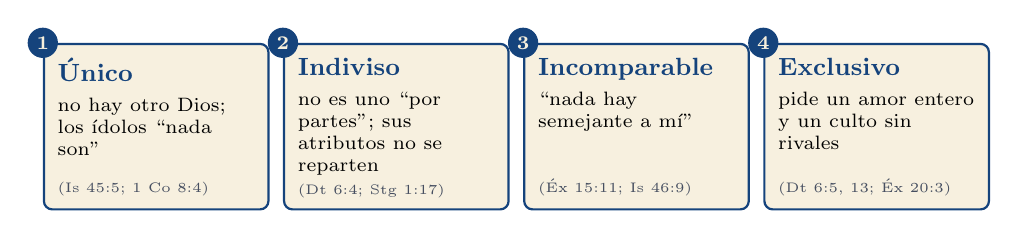
\begin{tikzpicture}
 \foreach \x/\n/\t/\d/\r in {0/1/{Único}/{no hay otro Dios; los ídolos ``nada son''}/{Is 45:5; 1~Co 8:4}, 3.05/2/{Indiviso}/{no es uno ``por partes''; sus atributos no se reparten}/{Dt 6:4; Stg 1:17}, 6.1/3/{Incomparable}/{``nada hay semejante a mí''}/{Éx 15:11; Is 46:9}, 9.15/4/{Exclusivo}/{pide un amor entero y un culto sin rivales}/{Dt 6:5, 13; Éx 20:3}}{
  \node[caja,anchor=north] (b\n) at (\x,0) {\parbox[t][1.75cm][t]{2.5cm}{\RaggedRight
    {\small\textbf{\textcolor{azul}{\t}}}\\[3pt]\scriptsize \d\par\vfill{\tiny\color{gris}(\r)}}};
  \node[circle,fill=azul,text=papiro,font=\scriptsize\bfseries,inner sep=1.6pt] at (b\n.north west) {\n};}
\end{tikzpicture}
\end{frame}

\begin{frame}{Uno, pero no ``uno de muchos''}
\begin{columns}[t,onlytextwidth]
\begin{column}{0.52\textwidth}\small
\begin{itemize}
\item Dios no es ``el mayor de los dioses'', como Baal o Marduk en sus panteones: es el \destacar{único} que existe como Dios (Sal 96:5).
\item Tampoco es uno como una especie (muchos individuos) o como un cuerpo (muchas partes).
\item Sus atributos no son piezas: el Santo es el Misericordioso, el Justo es el Fiel. Por eso la gloria de Dios es la \destacar{comunión} de todos ellos (tesis de esta obra).
\end{itemize}
\begin{cita}[fontupper=\scriptsize\itshape]Porque todos los dioses de los pueblos son ídolos; pero \SENOR{} hizo los cielos.\fuente{(Sal 96:5, RVR1960)}\end{cita}
\end{column}
\begin{column}{0.46\textwidth}
\begin{cita}[colback=dorado!10!papiro,colframe=dorado!80!azul,fontupper=\scriptsize\itshape]Este Dios es uno, y no dos ni más de dos, sino uno; cuya unidad no se parece a ninguna de las unidades que hay en el mundo: no es uno como una especie, que abarca muchos individuos, ni uno como un cuerpo, que se divide en partes y extremos.\fuente{(Maimónides, \emph{Yesodé haTorá} 1:7)}\end{cita}
\precision{la ``simplicidad'' de Dios es un término teológico, no bíblico; Maimónides concluye su párrafo citando Dt 6:4.}
\end{column}
\end{columns}
\end{frame}

\begin{frame}{Uno y, sin embargo, Padre, Hijo y Espíritu}
\begin{columns}[c,onlytextwidth]
\begin{column}{0.50\textwidth}\small
\begin{itemize}
\item La fe cristiana no corrige el \emph{Shemá}: lo confiesa. Jesús lo cita como ``el primer mandamiento de todos'' (Mr 12:29).
\item Dios es uno ``en la unidad de su naturaleza'', aunque subsistiendo en tres personas, como dice Pink (2020, cap. 1).
\item Pablo no añade un segundo Dios: incluye a Jesús \destacar{dentro} del único Dios del \emph{Shemá} (1~Co 8:6; ver ``En Cristo'').
\end{itemize}
\end{column}
\begin{column}{0.48\textwidth}
\centering
\begin{tikzpicture}[font=\scriptsize]
 \node[draw=dorado,line width=1.4pt,fill=azul,text=papiro,circle,minimum size=1.7cm,align=center] (u) at (0,0) {\heb{אֶחָד}\\ un solo Dios};
 \node[caja,text width=1.7cm,align=center] (p) at (0,2.0) {Padre\\ {\tiny 1~Co 8:6}};
 \node[caja,text width=1.7cm,align=center] (h) at (-1.9,-1.4) {Hijo\\ {\tiny Jn 1:18; Col 2:9}};
 \node[caja,text width=1.7cm,align=center] (e) at (1.9,-1.4) {Espíritu\\ {\tiny 1~Co 12:4--6}};
 \foreach \n in {p,h,e}\draw[dorado,line width=1.2pt] (u)--(\n);
 \node[text width=4.2cm,align=center,font=\tiny,text=gris] at (0,-2.6) {``un cuerpo, y un Espíritu\ldots{} un Señor\ldots{} un Dios y Padre de todos'' (Ef 4:4--6)};
\end{tikzpicture}
\end{column}
\end{columns}\par\smallskip
\precision{la doctrina de la Trinidad es la formulación de la iglesia (siglos IV--V) a partir de estos textos; el judaísmo la rechaza como contraria al \emph{Shemá}. Aquí se expone la lectura cristiana sin atribuirla a las fuentes judías.}
\end{frame}

% ------------------------------------------------------------------
\section{Torá y Profetas}

\begin{frame}{``No tendrás dioses ajenos''}
\begin{columns}[t,onlytextwidth]
\begin{column}{0.50\textwidth}
\begin{center}\small\heb{לֹא יִהְיֶה לְךָ אֱלֹהִים אֲחֵרִים עַל־פָּנָי}\end{center}
\begin{cita}Yo soy \SENOR{} tu Dios, que te saqué de la tierra de Egipto, de casa de servidumbre. No tendrás dioses ajenos delante de mí.\fuente{(Éx 20:2--3, RVR1960)}\end{cita}
\end{column}
\begin{column}{0.48\textwidth}\small
\begin{itemize}
\item La unidad de Dios llega primero como \destacar{relación}: ``\emph{tu} Dios, que \emph{te} saqué''. No es una tesis, es un rescate.
\item \heb{אֱלֹהִים אֲחֵרִים}: ``otros dioses''. \heb{עַל־פָּנָי}: ``delante de mi rostro'', en mi presencia.
\item El \emph{Shemá} (Dt 6:4) es la forma positiva de este mandamiento.
\end{itemize}
\end{column}
\end{columns}
\end{frame}

\begin{frame}{``A ti te fue mostrado''}
\begin{columns}[t,onlytextwidth]
\begin{column}{0.52\textwidth}
\begin{center}\scriptsize\heb{אַתָּה הָרְאֵתָ לָדַעַת כִּי יְהוָה הוּא הָאֱלֹהִים אֵין עוֹד מִלְבַדּוֹ}\end{center}
\begin{cita}[fontupper=\scriptsize\itshape]A ti te fue mostrado, para que supieses que \SENOR{} es Dios, y no hay otro fuera de él.\fuente{(Dt 4:35, RVR1960)}\end{cita}
\begin{cita}[fontupper=\scriptsize\itshape]Aprende pues, hoy, y reflexiona en tu corazón que \SENOR{} es Dios arriba en el cielo y abajo en la tierra, y no hay otro.\fuente{(Dt 4:39, RVR1960)}\end{cita}
\end{column}
\begin{column}{0.46\textwidth}\small
\begin{itemize}
\item Israel no deduce la unidad de Dios: la \destacar{vio} en el éxodo y en el Horeb (Dt 4:32--38).
\item En el Horeb oyó una voz, pero ``ninguna figura visteis'' (4:12, 15): el Uno no tiene imagen.
\item \heb{יְהוָה הוּא הָאֱלֹהִים}: ``\SENOR{} es \emph{el} Dios''. Es la misma frase que gritará el pueblo en el Carmelo (1~R 18:39).
\end{itemize}
\end{column}
\end{columns}
\end{frame}

\begin{frame}{Isaías: los testigos del Uno}
\begin{columns}[t,onlytextwidth]
\begin{column}{0.50\textwidth}
\begin{cita}[fontupper=\scriptsize\itshape]Vosotros sois mis testigos, dice \SENOR, y mi siervo que yo escogí, para que me conozcáis y creáis, y entendáis que yo mismo soy; antes de mí no fue formado dios, ni lo será después de mí. Yo, yo \SENOR, y fuera de mí no hay quien salve.\fuente{(Is 43:10--11, RVR1960)}\end{cita}
\begin{cita}[fontupper=\scriptsize\itshape]Mirad a mí, y sed salvos, todos los términos de la tierra, porque yo soy Dios, y no hay más.\fuente{(Is 45:22, RVR1960)}\end{cita}
\end{column}
\begin{column}{0.48\textwidth}\small
\begin{itemize}
\item En el exilio, Babilonia parecía probar que Marduk era más fuerte. Isaías convoca un \destacar{juicio}: que los dioses anuncien el futuro (41:21--24).
\item Israel es el testigo (\heb{עֵדַי}, 43:10): la nación entera es una \heb{עֵד} viva.
\item El monoteísmo de Isaías es \destacar{misionero}: ``todos los términos de la tierra'' (45:22).
\end{itemize}
\end{column}
\end{columns}
\end{frame}

\begin{frame}{Un mismo Padre, un mismo Dios}
\begin{columns}[c,onlytextwidth]
\begin{column}{0.52\textwidth}
\begin{center}\small\heb{הֲלוֹא אָב אֶחָד לְכֻלָּנוּ הֲלוֹא אֵל אֶחָד בְּרָאָנוּ}\end{center}
\begin{cita}¿No tenemos todos un mismo padre? ¿No nos ha creado un mismo Dios? ¿Por qué, pues, nos portamos deslealmente el uno contra el otro, profanando el pacto de nuestros padres?\fuente{(Mal 2:10, RVR1960)}\end{cita}
\end{column}
\begin{column}{0.46\textwidth}\small
\begin{itemize}
\item Malaquías saca la consecuencia \destacar{ética}: si Dios es uno, sus hijos no pueden traicionarse entre sí.
\item La unidad de Dios funda la unidad del pueblo: ``un rey será a todos ellos\ldots{} nunca más serán dos naciones'' (Ez 37:22).
\item ``Les daré un corazón, y un camino'' (Jer 32:39: \heb{לֵב אֶחָד וְדֶרֶךְ אֶחָד}).
\end{itemize}
\end{column}
\end{columns}
\end{frame}

% ------------------------------------------------------------------
\section{Teología}

\begin{frame}{``Dios está solo en su excelencia''}
\begin{columns}[t,onlytextwidth]
\begin{column}{0.54\textwidth}\small
Antes de crear, Dios no tenía con quién compararse ni de quién depender: estaba solo, completo y sin necesidad de nada. Por eso su unidad no es la de ``uno entre varios'', sino la de quien no tiene par. El cántico del mar lo dice en forma de pregunta: ``¿Quién como tú, oh \SENOR, entre los dioses?'' (Éx 15:11). Como resume Pink (2020, cap. 1), ``Dios está solo en su excelencia''.\par\smallskip
Crear no le añadió nada; lo hizo ``según el designio de su voluntad'' (Ef 1:11). Por eso nadie puede ponerse a su lado ni ponerlo en deuda.
\end{column}
\begin{column}{0.44\textwidth}
\begin{cita}[fontupper=\scriptsize\itshape]\ldots{} el bienaventurado y solo Soberano, Rey de reyes, y Señor de señores, el único que tiene inmortalidad, que habita en luz inaccesible\ldots\fuente{(1~Ti 6:15--16, RVR1960)}\end{cita}
\begin{cita}[fontupper=\scriptsize\itshape]¿O quién le dio a él primero, para que le fuese recompensado?\fuente{(Ro 11:35, RVR1960)}\end{cita}
\end{column}
\end{columns}
\end{frame}

\begin{frame}{Conocido solo por revelación}
\begin{columns}[c,onlytextwidth]
\begin{column}{0.52\textwidth}\small
Si Dios no tiene par, ninguna comparación lo alcanza: ``¿A qué, pues, haréis semejante a Dios, o qué imagen le compondréis?'' (Is 40:18). Lo que el hombre ve de él son apenas ``los bordes de sus caminos'' (Job 26:14), y el hombre natural ``no percibe las cosas que son del Espíritu de Dios'' (1~Co 2:14). El Dios único se conoce cuando él se \destacar{revela} por su Palabra y su Espíritu (Pink, 2020, cap. 1).\par\smallskip
Por eso el \emph{Shemá} empieza con ``oye'' y no con ``piensa''.
\end{column}
\begin{column}{0.46\textwidth}
\begin{cita}[fontupper=\scriptsize\itshape]Porque Dios, que mandó que de las tinieblas resplandeciese la luz, es el que resplandeció en nuestros corazones, para iluminación del conocimiento de la gloria de Dios en la faz de Jesucristo.\fuente{(2~Co 4:6, RVR1960)}\end{cita}
\end{column}
\end{columns}\par\smallskip
\precision{la relación entre la unicidad y el ``Shemá empieza con oye'' es observación propia.}
\end{frame}

% ------------------------------------------------------------------
\section{En Israel}

\begin{frame}{Elías en el Carmelo}
\fotolado{panel_1reyes18.jpg}{Elaboración propia: 1~R 18:39 en texto hebreo consonántico (BHS).}
\begin{columns}[c,onlytextwidth]
\begin{column}{0.58\textwidth}
\begin{center}\scriptsize\heb{עַד־מָתַי אַתֶּם פֹּסְחִים עַל־שְׁתֵּי הַסְּעִפִּים}\end{center}
\begin{cita}[fontupper=\scriptsize\itshape]Y acercándose Elías a todo el pueblo, dijo: ¿Hasta cuándo claudicaréis vosotros entre dos pensamientos? Si \SENOR{} es Dios, seguidle; y si Baal, id en pos de él. Y el pueblo no respondió palabra.\fuente{(1~R 18:21, RVR1960)}\end{cita}
\small Acab y Jezabel han instalado el culto de Baal en Israel (16:31--33). Tres años sin lluvia (18:1). En el monte, el pueblo quiere tener \destacar{dos dioses}: \SENOR{} y Baal.
\end{column}
\begin{column}{0.40\textwidth}\end{column}
\end{columns}
\end{frame}

\begin{frame}{``Claudicar entre dos''}
\scriptsize\renewcommand{\arraystretch}{1.15}
\begin{tabular}{@{}>{\RaggedRight\arraybackslash}p{2.9cm}>{\RaggedRight\arraybackslash}p{1.0cm}>{\RaggedRight\arraybackslash}p{7.9cm}@{}}
\toprule
\textbf{Término} & \textbf{Raíz} & \textbf{Sentido} \\ \midrule
\heb{פֹּסְחִים} \emph{posjim} (18:21) & \heb{פסח} & ``cojear, saltar'': la misma raíz describe la danza de los profetas de Baal ``saltando'' alrededor del altar (v.~26). \\
\heb{שְׁתֵּי הַסְּעִפִּים} (18:21) & \heb{סעף} & ``las dos ramas'' u ``opiniones'' (RVR1960: ``pensamientos''): el pueblo va de una a otra como quien no sabe en qué pie apoyarse. \\
\heb{אֵלִיָּהוּ} \emph{Eliyahu} & --- & el nombre del profeta es una confesión: ``mi Dios es \emph{Yah}''. \\
\heb{שְׁתֵּים עֶשְׂרֵה אֲבָנִים} (18:31) & --- & doce piedras ``conforme al número de las tribus'': un solo Dios, un solo pueblo, aunque el reino esté dividido. \\
\heb{יְהוָה הוּא הָאֱלֹהִים} (18:39) & --- & ``\SENOR{} es el Dios'': la frase de Dt 4:35, 39, repetida dos veces. \\
\bottomrule
\end{tabular}\par\medskip
\small Baal no responde: ``no hubo ninguna voz, ni quien respondiese ni escuchase'' (18:29). El Uno responde con fuego.
\end{frame}

\begin{frame}{``¡\SENOR{} es el Dios!''}
\begin{columns}[t,onlytextwidth]
\begin{column}{0.54\textwidth}
\begin{cita}[fontupper=\scriptsize\itshape]\SENOR{} Dios de Abraham, de Isaac y de Israel, sea hoy manifiesto que tú eres Dios en Israel\ldots{} Respóndeme, \SENOR, respóndeme, para que conozca este pueblo que tú, oh \SENOR, eres el Dios, y que tú vuelves a ti el corazón de ellos. Entonces cayó fuego de \SENOR, y consumió el holocausto, la leña, las piedras y el polvo, y aun lamió el agua que estaba en la zanja. Viéndolo todo el pueblo, se postraron y dijeron: ¡\SENOR{} es el Dios, \SENOR{} es el Dios!\fuente{(1~R 18:36--39, RVR1960)}\end{cita}
\end{column}
\begin{column}{0.44\textwidth}\small
\begin{itemize}
\item Elías no pide solo fuego: pide que Dios ``vuelva el corazón'' del pueblo. La unidad de Dios reclama un corazón no dividido.
\item El pueblo pasa del silencio (v.~21) a la confesión (v.~39).
\end{itemize}
\precision{el judaísmo cierra el Día de la Expiación (oración de \emph{Neilá}) diciendo una vez el \emph{Shemá}, tres veces ``Bendito sea el nombre\ldots'' y siete veces ``\SENOR{} es el Dios'' (\emph{Shulján Aruj}, Óraj Jayim 623:6).}
\end{column}
\end{columns}
\end{frame}

% ------------------------------------------------------------------
\section{Judaísmo}

\begin{frame}{Aceptar el yugo del Reino}
\begin{columns}[t,onlytextwidth]
\begin{column}{0.52\textwidth}
\begin{cita}[colback=dorado!10!papiro,colframe=dorado!80!azul,fontupper=\scriptsize\itshape]¿Por qué precede el \emph{Shemá} a ``Y será, si obedeciereis''? Para que uno acepte sobre sí primero el yugo del Reino de los cielos, y después acepte sobre sí el yugo de los mandamientos.\fuente{(Misná, \emph{Berajot} 2:2, R. Yehoshúa ben Qorjá)}\end{cita}
\begin{center}\scriptsize\heb{כְדֵי שֶׁיְּקַבֵּל עָלָיו עֹל מַלְכוּת שָׁמַיִם תְּחִלָּה}\end{center}
\end{column}
\begin{column}{0.46\textwidth}\small
\begin{itemize}
\item El judío recita el \emph{Shemá} (Dt 6:4--9; 11:13--21; Nm 15:37--41) por la mañana y por la noche: ``al acostarte, y cuando te levantes'' (Dt 6:7).
\item Confesar que Dios es uno es \destacar{someterse} a Él como Rey: primero el Reino, después los mandamientos.
\item El Targum Ónkelos traduce: \heb{יְיָ אֱלָהָנָא יְיָ חָד}.
\end{itemize}
\end{column}
\end{columns}
\end{frame}

\begin{frame}{Prolongar el ``uno''}
\begin{columns}[c,onlytextwidth]
\begin{column}{0.52\textwidth}
\begin{cita}[colback=dorado!10!papiro,colframe=dorado!80!azul,fontupper=\scriptsize\itshape]Símaco dice: todo el que prolonga el ``uno'', le prolongan sus días y sus años\ldots{} R. Yirmeyá vio que R. Jiyá bar Abbá lo prolongaba mucho, y le dijo: Una vez que lo has hecho Rey arriba, abajo y en los cuatro vientos del cielo, ya no hace falta más.\fuente{(\emph{Berajot} 13b)}\end{cita}
\end{column}
\begin{column}{0.46\textwidth}
\centering
\begin{tikzpicture}[font=\tiny]
 \node[draw=dorado,line width=1.4pt,fill=azul,text=papiro,circle,minimum size=1.2cm,align=center] (c) at (0,0) {\heb{אֶחָד}};
 \foreach \a/\t in {90/arriba,270/abajo,0/oriente,180/occidente,45/norte,225/sur}{
   \node[caja,inner sep=2pt] at (\a:1.55) {\t};}
 \node[text width=3.8cm,align=center,font=\tiny,text=gris] at (0,-2.4) {R. Ajá bar Yaakov: ``y en la \emph{dálet}'' (13b)};
\end{tikzpicture}
\end{column}
\end{columns}\par\smallskip
\small Decir \emph{ejad} es \destacar{proclamar rey} a Dios en todas las direcciones del mundo: nada queda fuera de su reinado.
\end{frame}

\begin{frame}{Jacob y sus hijos}
\begin{columns}[t,onlytextwidth]
\begin{column}{0.54\textwidth}
\begin{cita}[colback=dorado!10!papiro,colframe=dorado!80!azul,fontupper=\scriptsize\itshape]Jacob quiso revelar a sus hijos el fin de los días, y la Presencia se apartó de él. Dijo: ¿Habrá en mi lecho algo defectuoso, como Abraham, de quien salió Ismael, y mi padre Isaac, de quien salió Esaú? Le dijeron sus hijos: ``Oye, Israel: \SENOR{} nuestro Dios, \SENOR{} uno es''. Dijeron: así como en tu corazón no hay sino uno, así en nuestro corazón no hay sino uno. En aquella hora Jacob dijo: ``Bendito sea el nombre de la gloria de su reino por siempre jamás''.\fuente{(\emph{Pesajim} 56a, R. Shimón ben Laquish)}\end{cita}
\end{column}
\begin{column}{0.44\textwidth}\small
\begin{itemize}
\item ``Israel'' en el \emph{Shemá} es leído como \destacar{Jacob}: los doce hijos confiesan al padre el Dios de su padre (Gn 49:2).
\item De ahí la línea que se dice en voz baja tras el primer verso: \heb{בָּרוּךְ שֵׁם כְּבוֹד מַלְכוּתוֹ לְעוֹלָם וָעֶד}.
\item ``En nuestro corazón no hay sino uno'': la unidad de Dios produce la unidad de la familia.
\end{itemize}
\precision{midrash talmúdico; también en \emph{Sifré Devarim} 31.}
\end{column}
\end{columns}
\end{frame}

\begin{frame}{En el mar y en el Sinaí: el mismo}
\begin{columns}[t,onlytextwidth]
\begin{column}{0.52\textwidth}
\begin{cita}[colback=dorado!10!papiro,colframe=dorado!80!azul,fontupper=\scriptsize\itshape]``Yo soy \SENOR{} tu Dios'': ¿por qué se dijo? Porque se reveló en el mar como un guerrero que hace guerras, y se reveló en el monte Sinaí como un anciano lleno de misericordia. Para no dar pretexto a las naciones del mundo de decir: ¡son dos poderes!\ldots{} Yo en Egipto, yo en el mar, yo en el Sinaí; yo en el pasado, yo en el porvenir.\fuente{(\emph{Mejiltá de R. Yishmael}, Bajódesh 5)}\end{cita}
\end{column}
\begin{column}{0.46\textwidth}\small
\begin{itemize}
\item Los rostros de Dios cambian (guerrero, anciano), pero Dios \destacar{no se divide}: es el mismo en la ira y en la misericordia.
\item Isaías dice lo mismo: ``yo \SENOR, el primero, y yo mismo con los postreros'' (Is 41:4).
\item Es la regla de lectura de toda esta serie: los atributos no son dioses distintos, son el único Dios.
\end{itemize}
\precision{el midrash responde a la idea de ``dos poderes en el cielo'', discutida por los sabios (Segal, 1977).}
\end{column}
\end{columns}
\end{frame}

\begin{frame}{``Con todo tu corazón''}
\begin{columns}[t,onlytextwidth]
\begin{column}{0.50\textwidth}
\begin{cita}[colback=dorado!10!papiro,colframe=dorado!80!azul,fontupper=\scriptsize\itshape]``Con todo tu corazón'': con tus dos inclinaciones, la buena y la mala. ``Con toda tu alma'': aunque te quite el alma. ``Con todas tus fuerzas'': con todo tu dinero.\fuente{(Misná, \emph{Berajot} 9:5)}\end{cita}
\begin{center}\scriptsize\heb{בְּכָל לְבָבְךָ בִּשְׁנֵי יְצָרֶיךָ}\end{center}
\end{column}
\begin{column}{0.48\textwidth}\small
\begin{itemize}
\item La Misná lee \heb{לְבָבְךָ} con dos \heb{ב} (\emph{levavjá}, no \emph{libjá}): dos inclinaciones que deben amar a un solo Dios.
\item El corazón dividido se \destacar{unifica} cuando las dos inclinaciones sirven al Uno (Sal 86:11).
\item ``Con toda tu alma'' prepara el relato de R. Akiva (ver también ``Dios es amor'').
\end{itemize}
\end{column}
\end{columns}
\end{frame}

\begin{frame}{R. Akiva: morir en el ``uno''}
\begin{columns}[c,onlytextwidth]
\begin{column}{0.54\textwidth}
\begin{cita}[colback=dorado!10!papiro,colframe=dorado!80!azul,fontupper=\scriptsize\itshape]Cuando sacaron a R. Akiva para matarlo, era la hora de recitar el \emph{Shemá}; le rastrillaban la carne con peines de hierro, y él aceptaba sobre sí el yugo del Reino de los cielos\ldots{} Prolongó el ``uno'' hasta que su alma salió en el ``uno''.\fuente{(\emph{Berajot} 61b)}\end{cita}
\begin{center}\scriptsize\heb{הָיָה מַאֲרִיךְ בְּאֶחָד עַד שֶׁיָּצְתָה נִשְׁמָתוֹ בְּאֶחָד}\end{center}
\end{column}
\begin{column}{0.44\textwidth}\small
\begin{itemize}
\item Roma, tras la rebelión de Bar Kojba (s.~II), prohíbe estudiar la Torá.
\item Akiva había esperado toda la vida cumplir ``con toda tu alma, aunque te quite el alma''.
\item El \emph{Shemá} se volvió la última palabra de los mártires judíos: confesar al Uno hasta la muerte. (El relato completo, en ``Dios es amor''.)
\end{itemize}
\end{column}
\end{columns}
\end{frame}

\begin{frame}{Qumrán: el \emph{Shemá} en filacterias}
\begin{columns}[t,onlytextwidth]
\begin{column}{0.52\textwidth}\small
\begin{itemize}
\item En las cuevas de Qumrán aparecieron filacterias (\emph{tefilín}) y \emph{mezuzot} con Dt 6:4--9: la orden de ``atarlas'' y ``escribirlas'' (6:8--9) se cumplía literalmente (Milik, 1977).
\item El Papiro Nash (Egipto, s.~II--I a.\,e.\,c.) contiene el Decálogo seguido del \emph{Shemá}, con una frase introductoria que coincide con la LXX (Burkitt, 1903).
\end{itemize}
\end{column}
\begin{column}{0.46\textwidth}
\begin{cita}[fontupper=\scriptsize\itshape]Y las atarás como una señal en tu mano, y estarán como frontales entre tus ojos; y las escribirás en los postes de tu casa, y en tus puertas.\fuente{(Dt 6:8--9, RVR1960)}\end{cita}
\precision{el Papiro Nash no es de Qumrán. La LXX de Dt 6:4 comienza: \grc{καὶ ταῦτα τὰ δικαιώματα καὶ τὰ κρίματα}, ``y estos son los estatutos y los decretos''. Conviene cotejar las filacterias en la Leon Levy Dead Sea Scrolls Digital Library.}
\end{column}
\end{columns}
\end{frame}

% ------------------------------------------------------------------
\section{En Cristo}

\begin{frame}{Jesús y el \emph{Shemá}}
\begin{columns}[c,onlytextwidth]
\begin{column}{0.54\textwidth}
\begin{cita}[fontupper=\scriptsize\itshape]Jesús le respondió: El primer mandamiento de todos es: Oye, Israel; el Señor nuestro Dios, el Señor uno es. Y amarás al Señor tu Dios con todo tu corazón, y con toda tu alma, y con toda tu mente y con todas tus fuerzas\ldots{} Entonces el escriba le dijo: Bien, Maestro, verdad has dicho, que uno es Dios, y no hay otro fuera de él.\fuente{(Mr 12:29--30, 32, RVR1960)}\end{cita}
\end{column}
\begin{column}{0.44\textwidth}\small
\begin{itemize}
\item Jesús, judío, empieza por el \emph{Shemá}: \grc{κύριος εἷς ἐστιν}, palabra por palabra de la LXX.
\item El escriba añade Dt 4:35: ``no hay otro fuera de él''.
\item Jesús une el \emph{Shemá} con Lv 19:18: el amor al único Dios se prueba en el prójimo.
\end{itemize}
\end{column}
\end{columns}
\end{frame}

\begin{frame}{1~Co 8:6: el \emph{Shemá} en Cristo}
\fotolado{panel_1corintios8.jpg}{Elaboración propia: 1~Co 8:6 en escritura uncial (texto NA28), con los \emph{nomina sacra} \grc{ΘΣ}, \grc{ΚΣ}, \grc{ΙΣ ΧΣ}.}
\begin{columns}[c,onlytextwidth]
\begin{column}{0.58\textwidth}
\begin{cita}[fontupper=\scriptsize\itshape]Acerca, pues, de las viandas que se sacrifican a los ídolos, sabemos que un ídolo nada es en el mundo, y que no hay más que un Dios. Pues aunque haya algunos que se llamen dioses\ldots{} para nosotros, sin embargo, sólo hay un Dios, el Padre, del cual proceden todas las cosas, y nosotros somos para él; y un Señor, Jesucristo, por medio del cual son todas las cosas, y nosotros por medio de él.\fuente{(1~Co 8:4--6, RVR1960)}\end{cita}
\scriptsize Corinto: carne sacrificada a los ídolos. Pablo responde con el \emph{Shemá}, pero lo confiesa de un modo nuevo.
\end{column}
\begin{column}{0.40\textwidth}\end{column}
\end{columns}
\end{frame}

\begin{frame}{Un Dios, un Señor}
\centering
\begin{tikzpicture}[font=\scriptsize]
 \node[font=\small\bfseries,text=azul] at (0,2.4) {Dt 6:4 LXX};
 \node[caja,text width=1.5cm,align=center] (k1) at (-3.6,1.6) {\grc{κύριος}\\ Señor};
 \node[caja,text width=1.5cm,align=center] (t) at (-1.2,1.6) {\grc{ὁ θεὸς ἡμῶν}\\ nuestro Dios};
 \node[caja,text width=1.5cm,align=center] (k2) at (1.2,1.6) {\grc{κύριος}\\ Señor};
 \node[caja,text width=1.5cm,align=center] (h) at (3.6,1.6) {\grc{εἷς}\\ uno};
 \node[font=\small\bfseries,text=azul] at (0,-0.15) {1~Co 8:6};
 \node[draw=dorado,line width=1.4pt,fill=azul,text=papiro,rounded corners=3pt,text width=4.3cm,align=center] (a) at (-2.6,-1.0) {\grc{εἷς θεὸς ὁ πατήρ}\\ un Dios, el Padre: \emph{de} quien todo};
 \node[draw=dorado,line width=1.4pt,fill=azul,text=papiro,rounded corners=3pt,text width=4.3cm,align=center] (b) at (2.6,-1.0) {\grc{εἷς κύριος Ἰησοῦς Χριστός}\\ un Señor, Jesucristo: \emph{por} quien todo};
 \draw[-{Latex[length=2mm]},dorado,line width=1.1pt] (t)--(a);
 \draw[-{Latex[length=2mm]},dorado,line width=1.1pt] (h)--(a);
 \draw[-{Latex[length=2mm]},dorado,line width=1.1pt] (k2)--(b);
 \draw[-{Latex[length=2mm]},dorado,line width=1.1pt] (h)--(b);
\end{tikzpicture}\par\medskip
\begin{columns}[t,onlytextwidth]
\begin{column}{0.52\textwidth}\small
Pablo reparte las palabras del \emph{Shemá}: ``Dios'' para el Padre y ``Señor'' (\grc{κύριος}, el griego para el Nombre) para Jesús. No suma un segundo Dios: pone a Jesús \destacar{dentro} de la confesión del único Dios, como mediador de la creación.
\end{column}
\begin{column}{0.46\textwidth}
\precision{lectura propuesta por Wright (1991) y Bauckham (2008), extendida en la exégesis actual; otros intérpretes ven solo un paralelo. Es interpretación cristiana, no judía.}
\end{column}
\end{columns}
\end{frame}

\begin{frame}{Un Dios, un pueblo}
\begin{columns}[t,onlytextwidth]
\begin{column}{0.50\textwidth}
\begin{cita}[fontupper=\scriptsize\itshape]¿Es Dios solamente Dios de los judíos? ¿No es también Dios de los gentiles? Ciertamente, también de los gentiles. Porque Dios es uno, y él justificará por la fe a los de la circuncisión, y por medio de la fe a los de la incircuncisión.\fuente{(Ro 3:29--30, RVR1960)}\end{cita}
\begin{cita}[fontupper=\scriptsize\itshape]Porque no hay diferencia entre judío y griego, pues el mismo que es Señor de todos, es rico para con todos los que le invocan.\fuente{(Ro 10:12, RVR1960)}\end{cita}
\end{column}
\begin{column}{0.48\textwidth}\small
\begin{itemize}
\item \grc{εἴπερ εἷς ὁ θεός}: el argumento de Pablo es el \emph{Shemá}. Si Dios es uno, no puede tener dos pueblos ni dos caminos de justificación.
\item Es el \emph{Sifré} al revés: lo que el midrash esperaba para ``el mundo venidero'' (\SENOR{} uno sobre todos), Pablo lo ve cumplido en el evangelio.
\item Zac 14:9 empieza a cumplirse cuando judíos y gentiles invocan el mismo Nombre (Ro 10:13 = Jl 2:32).
\end{itemize}
\end{column}
\end{columns}
\end{frame}

\begin{frame}{Siete ``uno''}
\begin{columns}[c,onlytextwidth]
\begin{column}{0.48\textwidth}
\begin{cita}[fontupper=\scriptsize\itshape]solícitos en guardar la unidad del Espíritu en el vínculo de la paz; un cuerpo, y un Espíritu, como fuisteis también llamados en una misma esperanza de vuestra vocación; un Señor, una fe, un bautismo, un Dios y Padre de todos, el cual es sobre todos, y por todos, y en todos.\fuente{(Ef 4:3--6, RVR1960)}\end{cita}
\scriptsize Ef 2:14--16: Cristo ``de ambos pueblos hizo uno'', ``un solo y nuevo hombre''.
\end{column}
\begin{column}{0.50\textwidth}
\centering
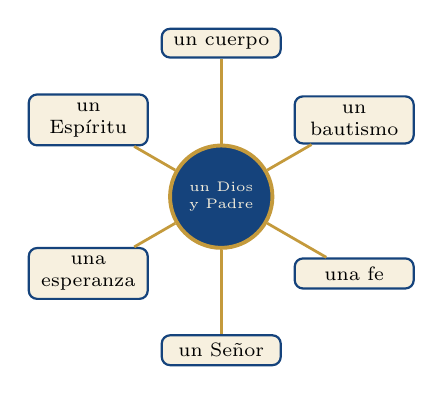
\begin{tikzpicture}[font=\tiny]
 \node[draw=dorado,line width=1.4pt,fill=azul,text=papiro,circle,minimum size=1.3cm,align=center] (d) at (0,0) {un Dios\\ y Padre};
 \foreach \a/\t in {90/{un cuerpo},150/{un Espíritu},210/{una esperanza},270/{un Señor},330/{una fe},30/{un bautismo}}{
   \node[caja,inner sep=3pt,text width=1.3cm,align=center] (n\a) at (\a:1.95) {\t};
   \draw[dorado,line width=1pt] (d)--(n\a);}
\end{tikzpicture}\par\smallskip
\small La unidad de la iglesia no es una meta humana: se \destacar{guarda} porque nace del Dios uno.
\end{column}
\end{columns}
\end{frame}

\begin{frame}{Toda rodilla: Is 45 en Flp 2}
\begin{columns}[t,onlytextwidth]
\begin{column}{0.50\textwidth}
\begin{cita}[fontupper=\scriptsize\itshape]Mirad a mí, y sed salvos, todos los términos de la tierra, porque yo soy Dios, y no hay más. Por mí mismo hice juramento\ldots{} Que a mí se doblará toda rodilla, y jurará toda lengua.\fuente{(Is 45:22--23, RVR1960)}\end{cita}
\begin{cita}[fontupper=\scriptsize\itshape]para que en el nombre de Jesús se doble toda rodilla\ldots{} y toda lengua confiese que Jesucristo es el Señor, para gloria de Dios Padre.\fuente{(Flp 2:10--11, RVR1960)}\end{cita}
\end{column}
\begin{column}{0.48\textwidth}\small
\begin{itemize}
\item Pablo toma el texto más fuerte del monoteísmo de Isaías (``no hay más'') y lo aplica a Jesús.
\item El ``nombre que es sobre todo nombre'' (Flp 2:9) es el Nombre del Uno: Zac 14:9 se cumple en la confesión ``Jesucristo es el Señor''.
\item Y todo termina ``para gloria de Dios Padre'': la unidad no se rompe.
\end{itemize}
\precision{lectura de Bauckham (2008); también Ro 14:11 cita Is 45:23.}
\end{column}
\end{columns}
\end{frame}

\begin{frame}{La plenitud del Uno en Cristo}
\centering
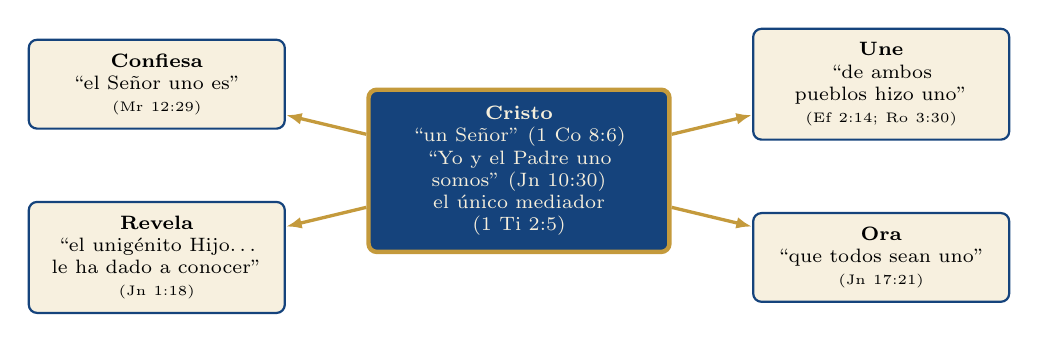
\begin{tikzpicture}[font=\scriptsize]
 \node[caja,text width=2.9cm,align=center] (a) at (-4.6,1.1) {\textbf{Confiesa}\\ ``el Señor uno es''\\ {\tiny(Mr 12:29)}};
 \node[caja,text width=2.9cm,align=center] (b) at (-4.6,-1.1) {\textbf{Revela}\\ ``el unigénito Hijo\ldots{} le ha dado a conocer''\\ {\tiny(Jn 1:18)}};
 \node[caja,text width=2.9cm,align=center] (c) at (4.6,1.1) {\textbf{Une}\\ ``de ambos pueblos hizo uno''\\ {\tiny(Ef 2:14; Ro 3:30)}};
 \node[caja,text width=2.9cm,align=center] (d) at (4.6,-1.1) {\textbf{Ora}\\ ``que todos sean uno''\\ {\tiny(Jn 17:21)}};
 \node[draw=dorado,line width=1.6pt,fill=azul,text=papiro,rounded corners=3pt,text width=3.4cm,align=center,inner sep=6pt] (x) at (0,0) {\textbf{Cristo}\\ ``un Señor'' (1~Co 8:6)\\ ``Yo y el Padre uno somos'' (Jn 10:30)\\ el único mediador (1~Ti 2:5)};
 \foreach \n in {a,b,c,d}\draw[dorado,line width=1.2pt,-{Latex[length=2mm]}] (x)--(\n);
\end{tikzpicture}\par\medskip
\small ``En él habita corporalmente toda la plenitud de la Deidad'' (Col 2:9): el Uno no se divide en Cristo; en Cristo se da a conocer.\par\smallskip
\precision{en Jn 10:30 ``uno'' es neutro (\grc{ἕν}): ``una sola cosa'', no ``una sola persona''. Juan, 1~Timoteo y Colosenses no son de Pablo o tienen autoría discutida; la idea paulina central está en 1~Co 8:6.}
\end{frame}

% ------------------------------------------------------------------
\section{Vivirlo}

\begin{frame}{Cinco consecuencias}
\scriptsize\renewcommand{\arraystretch}{1.22}
\begin{tabular}{@{}>{\RaggedRight\arraybackslash}p{2.4cm}>{\RaggedRight\arraybackslash}p{6.2cm}>{\RaggedRight\arraybackslash}p{3.3cm}@{}}
\toprule
\textbf{Actitud} & \textbf{Qué implica} & \textbf{Texto} \\ \midrule
\destacar{No claudicar} & no repartir el corazón entre Dios y otros ``dioses'' (dinero, prestigio, poder) & 1~R 18:21; Mt 6:24 \\
\destacar{Un corazón unido} & pedir lo que el salmista pidió: ``unifica mi corazón'' & Sal 86:11; Dt 6:5 \\
\destacar{Oír cada día} & hacer del \emph{Shemá} un hábito: en casa, en el camino, al acostarse y al levantarse & Dt 6:6--9 \\
\destacar{Guardar la unidad} & la iglesia dividida contradice a su Dios uno & Ef 4:3--6; Jn 17:21 \\
\destacar{Ser testigos} & llevar el Nombre del Uno a todas las naciones & Is 43:10; 45:22; Ro 3:29 \\
\bottomrule
\end{tabular}\par\medskip
\begin{cita}Y esta es la vida eterna: que te conozcan a ti, el único Dios verdadero, y a Jesucristo, a quien has enviado.\fuente{(Jn 17:3, RVR1960)}\end{cita}
\end{frame}

\begin{frame}{``Los demonios creen, y tiemblan''}
\begin{columns}[c,onlytextwidth]
\begin{column}{0.50\textwidth}
\begin{cita}Tú crees que Dios es uno; bien haces. También los demonios creen, y tiemblan.\fuente{(Stg 2:19, RVR1960)}\end{cita}
\begin{cita}[fontupper=\scriptsize\itshape]Ninguno puede servir a dos señores\ldots{}\fuente{(Mt 6:24a, RVR1960)}\end{cita}
\end{column}
\begin{column}{0.48\textwidth}\small
\begin{itemize}
\item Santiago cita el \emph{Shemá} (\grc{εἷς ἐστιν ὁ θεός}) para advertir: se puede confesar la unidad de Dios con los labios y tener el corazón dividido.
\item El \emph{Shemá} no termina en el v.~4: sigue ``y amarás'' (v.~5). La ortodoxia sin amor es la fe de los demonios.
\end{itemize}
\end{column}
\end{columns}
\end{frame}

% ------------------------------------------------------------------
\section{Síntesis}

\begin{frame}{Síntesis}
\begin{tcolorbox}[colback=papiro,colframe=azul,boxrule=1pt,arc=3pt]
\footnotesize Dios es uno: no hay otro fuera de Él (Dt 4:35), no tiene igual (Is 46:9) ni se divide (Dt 6:4). Israel lo confiesa cada día en el \emph{Shemá} y lo espera para toda la tierra: ``\SENOR{} será uno, y uno su nombre'' (Zac 14:9). En el Carmelo el pueblo deja de claudicar entre dos (1~R 18:39); los sabios hacen del ``uno'' la aceptación del Reino y la última palabra de los mártires. Pablo confiesa el mismo \emph{Shemá} en Cristo, ``un Dios, el Padre\ldots{} y un Señor, Jesucristo'' (1~Co 8:6), y saca de él un solo pueblo de judíos y gentiles (Ro 3:30).
\end{tcolorbox}
\scriptsize\renewcommand{\arraystretch}{1.12}
\begin{tabular}{@{}>{\RaggedRight\arraybackslash}p{2.0cm}>{\RaggedRight\arraybackslash}p{9.8cm}@{}}
\toprule
\textbf{Mirada} & \textbf{Aporte} \\ \midrule
Torá y Nombre & Dt 6:4--9; 4:35, 39; Éx 20:3; Zac 14:9; \heb{אֶחָד}, \heb{לְבַד}, \heb{אֵין עוֹד}; Is 43--46; Mal 2:10; Sal 86:10--11. \\
Encuentro & Elías en el Carmelo (1~R 18): ``¡\SENOR{} es el Dios!''. \\
Judaísmo & \emph{Berajot} 2:2; 9:5; 13b; 61b; \emph{Pesajim} 56a; \emph{Sifré} 31; Rashi; \emph{Mejiltá}; Maimónides; \emph{Neilá}; filacterias. \\
Teológica & la unicidad de Dios: solo en su excelencia, conocido por revelación. \\
Paulina & 1~Co 8:4--6; Ro 3:29--30; 10:12; Gá 3:20; Ef 4:4--6; Flp 2:9--11. \\
\bottomrule
\end{tabular}
\end{frame}

\begin{frame}{Para la reflexión}
\begin{cita}Oye, Israel: \SENOR{} nuestro Dios, \SENOR{} uno es. Y amarás a \SENOR{} tu Dios de todo tu corazón, y de toda tu alma, y con todas tus fuerzas.\fuente{(Dt 6:4--5, RVR1960)}\end{cita}
\begin{center}\heb{שְׁמַע יִשְׂרָאֵל יְהוָה אֱלֹהֵינוּ יְהוָה אֶחָד}\end{center}
\small
\begin{itemize}
\item ¿Entre qué ``dos pensamientos'' estoy claudicando hoy (1~R 18:21)?
\item ¿Qué parte de mi corazón necesita ser ``unificada'' para temer su Nombre (Sal 86:11)?
\item ¿En qué momentos de mi día (al acostarme, al levantarme, en el camino) confieso que Dios es uno?
\item ¿Cómo vivo la unidad con hermanos distintos de mí, si Dios es uno (Ro 3:29--30; Ef 4:3)?
\end{itemize}
\end{frame}

% ------------------------------------------------------------------
\section{Glosario}

\begin{frame}{Glosario}
\scriptsize\RaggedRight
\begin{columns}[t,onlytextwidth]
\begin{column}{0.49\textwidth}

\par\noindent\hangindent=1em{\color{azul}\textbf{\emph{Alenu}}} oración que cierra los servicios judíos; termina con Zac 14:9.\par\vspace{2pt}
\par\noindent\hangindent=1em{\color{azul}\textbf{\emph{Ani hu}}} (\heb{אֲנִי הוּא}) ``yo soy'' (Dt 32:39; Is 43:10).\par\vspace{2pt}
\par\noindent\hangindent=1em{\color{azul}\textbf{\emph{Ed}}} (\heb{עֵד}) testigo; letras grandes de Dt 6:4.\par\vspace{2pt}
\par\noindent\hangindent=1em{\color{azul}\textbf{\emph{Ein od}}} (\heb{אֵין עוֹד}) ``no hay otro'' (Dt 4:35; Is 45:5).\par\vspace{2pt}
\par\noindent\hangindent=1em{\color{azul}\textbf{\emph{Ejad}}} (\heb{אֶחָד}) uno, uno solo, el mismo (Dt 6:4; Zac 14:9).\par\vspace{2pt}
\par\noindent\hangindent=1em{\color{azul}\textbf{\emph{Heîs}}} (\grc{εἷς}) uno (Mr 12:29; 1~Co 8:6).\par\vspace{2pt}
\par\noindent\hangindent=1em{\color{azul}\textbf{\emph{Levad}}} (\heb{לְבַד}) solo, aparte (Neh 9:6; Sal 86:10).\par\vspace{2pt}
\par\noindent\hangindent=1em{\color{azul}\textbf{\emph{Mónos}}} (\grc{μόνος}) solo, único (Jn 17:3; Ro 16:27).\par\vspace{2pt}

\end{column}
\begin{column}{0.49\textwidth}

\par\noindent\hangindent=1em{\color{azul}\textbf{\emph{Neilá}}} oración final del Día de la Expiación.\par\vspace{2pt}
\par\noindent\hangindent=1em{\color{azul}\textbf{\emph{Pasaj}}} (\heb{פסח}) cojear, saltar; ``claudicar'' (1~R 18:21).\par\vspace{2pt}
\par\noindent\hangindent=1em{\color{azul}\textbf{\emph{Shemá}}} (\heb{שְׁמַע}) ``oye''; nombre de Dt 6:4--9 y de la oración diaria.\par\vspace{2pt}
\par\noindent\hangindent=1em{\color{azul}\textbf{\emph{Tefilín}}} filacterias: cajitas con Dt 6:4--9 y otros textos (Dt 6:8).\par\vspace{2pt}
\par\noindent\hangindent=1em{\color{azul}\textbf{\emph{Ol maljut shamáyim}}} ``yugo del Reino de los cielos'' (Misná \emph{Berajot} 2:2).\par\vspace{2pt}
\par\noindent\hangindent=1em{\color{azul}\textbf{\emph{Yajed}}} (\heb{יַחֵד}) unificar (Sal 86:11).\par\vspace{2pt}
\par\noindent\hangindent=1em{\color{azul}\textbf{\emph{Yajid}}} (\heb{יָחִיד}) único, hijo único (Gn 22:2).\par\vspace{2pt}

\end{column}
\end{columns}
\end{frame}

% ------------------------------------------------------------------
\section{Referencias}

\begin{frame}{Referencias}
\fontsize{5.0}{6.0}\selectfont
\begin{columns}[t,onlytextwidth]
\begin{column}{0.49\textwidth}
\refapa{Bauckham, R. (2008). \emph{Jesus and the God of Israel: God crucified and other studies on the New Testament's christology of divine identity}. Eerdmans.}
\refapa{Block, D.~I. (2004). How many is God? An investigation into the meaning of Deuteronomy 6:4--5. \emph{Journal of the Evangelical Theological Society, 47}(2), 193--212.}
\refapa{Burkitt, F.~C. (1903). The Hebrew papyrus of the Ten Commandments. \emph{The Jewish Quarterly Review, 15}(3), 392--408.}
\refapa{Carson, D.~A. (2013). \emph{Falacias exegéticas}. Editorial CLIE.}
\refapa{Elbogen, I. (1993). \emph{Jewish liturgy: A comprehensive history} (R.~P. Scheindlin, Trad.). Jewish Publication Society.}
\refapa{Elliger, K., \& Rudolph, W. (Eds.). (1997). \emph{Biblia Hebraica Stuttgartensia} (5.ª ed.). Deutsche Bibelgesellschaft.}
\refapa{Jaffee, M. (Trad.). (2015). \emph{Sifré Devarim} [31]. Sefaria. https://www.sefaria.org}
\refapa{Maimónides. (s.f.). \emph{Mishné Torá: Yesodé haTorá} [1:7]. Sefaria. https://www.sefaria.org}
\refapa{\emph{Mejiltá de R. Yishmael} [Bajódesh 5]. (s.f.). Sefaria. https://www.sefaria.org}
\refapa{Meshel, Z. (2012). \emph{Kuntillet `Ajrud (Ḥorvat Teman): An Iron Age II religious site on the Judah--Sinai border}. Israel Exploration Society.}
\refapa{Milik, J.~T. (1977). \emph{Qumrân grotte 4.II: Tefillin, mezuzot et targums (4Q128--4Q157)} (Discoveries in the Judaean Desert VI). Clarendon Press.}
\refapa{\emph{Misná: Berajot} [2:2; 9:5]. (s.f.). Sefaria. https://www.sefaria.org}
\end{column}
\begin{column}{0.49\textwidth}
\refapa{Nestle, E., \& Aland, K. (Eds.). (2012). \emph{Novum Testamentum Graece} (28.ª ed.). Deutsche Bibelgesellschaft.}
\refapa{Pink, A.~W. (2020). \emph{Los atributos de Dios} (E. Rodríguez Cruz, Trad.). Chapel Library. (Obra original publicada en 1930)}
\refapa{Rahlfs, A., \& Hanhart, R. (Eds.). (2006). \emph{Septuaginta} (Ed. rev.). Deutsche Bibelgesellschaft.}
\refapa{Rashi. (s.f.). \emph{Comentario a la Torá} [Dt 6:4]. Sefaria. https://www.sefaria.org}
\refapa{\emph{Santa Biblia: Reina-Valera 1960}. (1960). Sociedades Bíblicas en América Latina.}
\refapa{Segal, A.~F. (1977). \emph{Two powers in heaven: Early rabbinic reports about Christianity and Gnosticism}. Brill.}
\refapa{\emph{Shulján Aruj: Óraj Jayim} [623:6]. (s.f.). Sefaria. https://www.sefaria.org}
\refapa{Steinsaltz, A. (Ed.). (2017). \emph{Koren Talmud Bavli: Edición William Davidson} [Berajot 13b; 61b; Pesajim 56a]. Sefaria. https://www.sefaria.org}
\refapa{Steinsaltz, A. (s.f.). \emph{The portion of ``Shema'' (Deuteronomy 6:4--8)}. Steinsaltz Center. https://steinsaltz.org/essay/shema/}
\refapa{Strong, J. (1890). \emph{The exhaustive concordance of the Bible}. Hunt \& Eaton.}
\refapa{\emph{Targum Ónkelos} [Deuteronomio 6:4]. (s.f.). Sefaria. https://www.sefaria.org}
\refapa{Washer, P. (2021). \emph{Conociendo al Dios vivo} (A. Ávila et al., Trad.). Editorial Legado Bautista Confesional.}
\refapa{Wright, N.~T. (1991). \emph{The climax of the covenant: Christ and the law in Pauline theology}. T\&T Clark.}
\end{column}
\end{columns}
\par\smallskip{\color{gris}Las citas bíblicas son de la Reina-Valera 1960; ``Jehová'' se reemplaza por \SENOR. Hebreo: BHS; griego: NA28 y LXX de Rahlfs-Hanhart. Fuentes judías: Sefaria, en traducción propia; lo rabínico se marca como \emph{precisión}. Conteos propios con la biblioteca del proyecto.}
\end{frame}

\end{document}
